\section{Muhammad Fahmi(1174021)}
\subsection{Intalasi Map Proxy}
\begin{enumerate}
    \item Disini kita bisa menggunakan CMD dan Ketikkan pip install MapProxy
    \hfill\break
    \begin{figure}[H]
		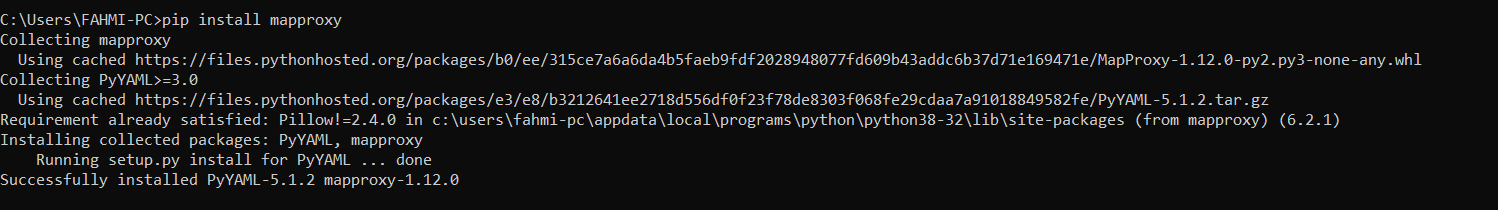
\includegraphics[width=4cm]{figures/1174021/5/1.png}
		\centering
		\caption{Perintah untuk menginstal map proxy}
    \end{figure}
\end{enumerate}

\subsection{Konfigurasi}
\begin{enumerate}
    \item Mari kita download filenya terlebih dahulu pada \href{https://github.com/awangga/gede}{Github Mr.Awangga}
    \hfill\break
    \begin{figure}[H]
		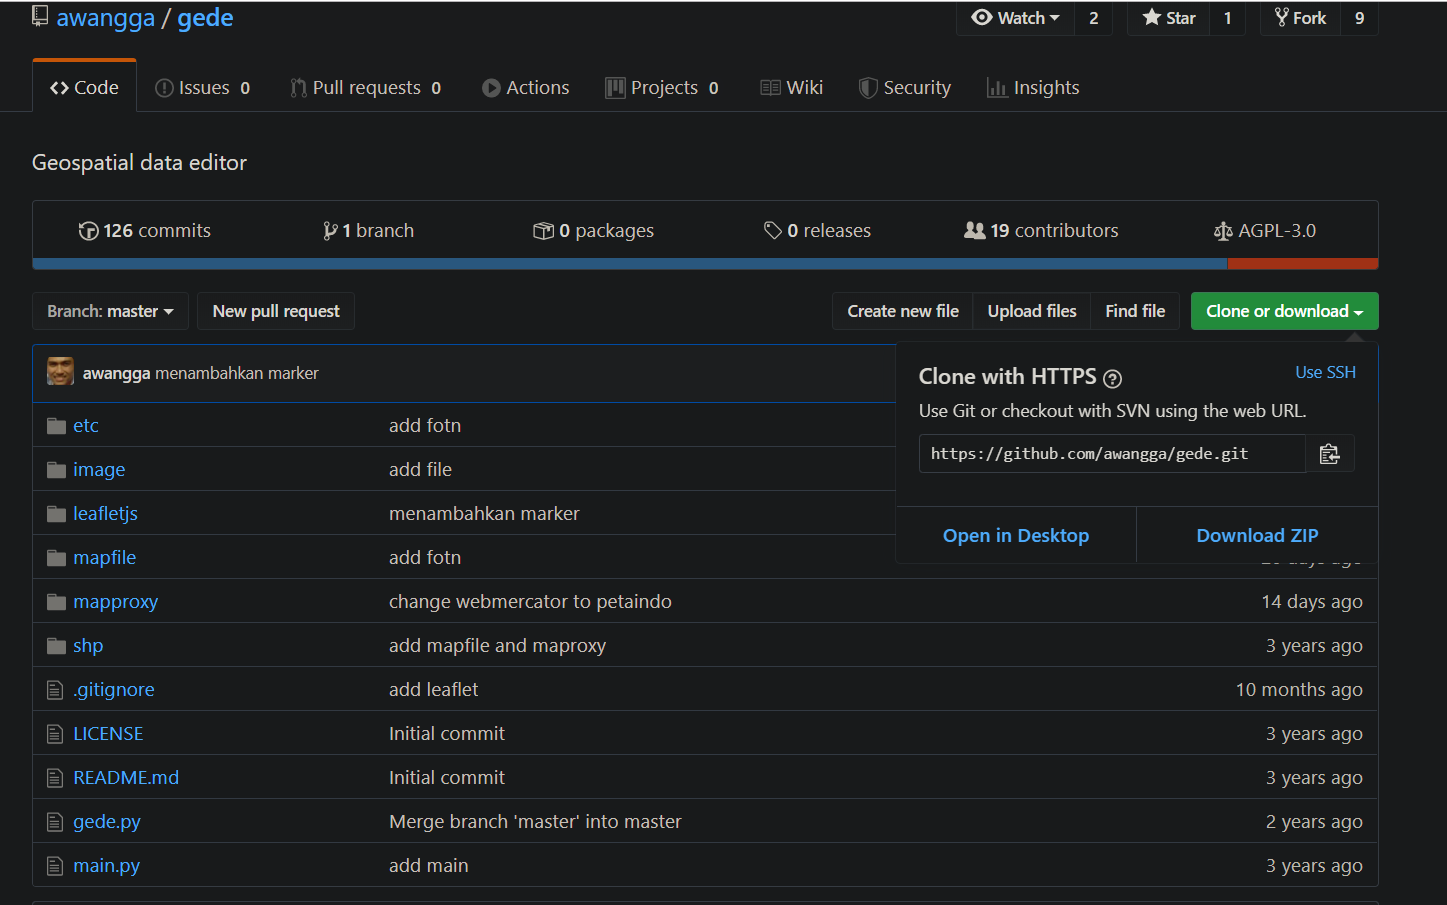
\includegraphics[width=4cm]{figures/1174021/5/2.png}
		\centering
		\caption{Download file untuk melakukan konfigurasi}
    \end{figure}

    \item Setelah didownload kemudian kita extrak
    \hfill\break
    \begin{figure}[H]
		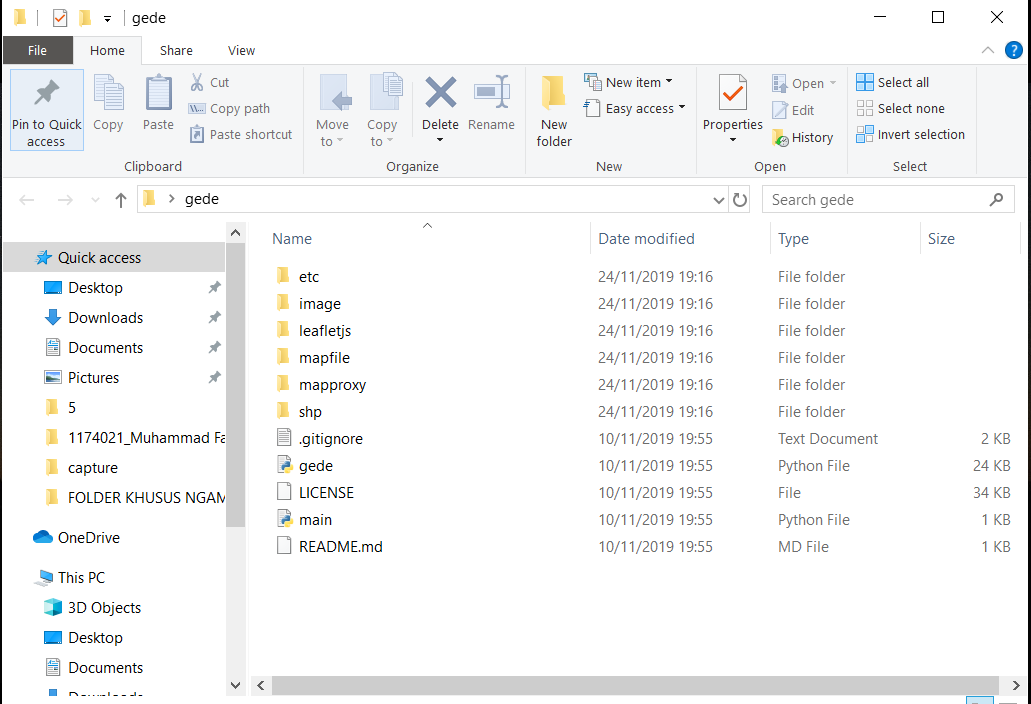
\includegraphics[width=4cm]{figures/1174021/5/3.png}
		\centering
		\caption{Extrack File Gede}
    \end{figure}

    \item Buka file agm.yaml, ubah map sesuai direktori file map, binari ubah sesuai direktori mapserver, working dir ubah sesuai direktori gede-master yang sebelumnya di download.
    \hfill\break
    \begin{figure}[H]
		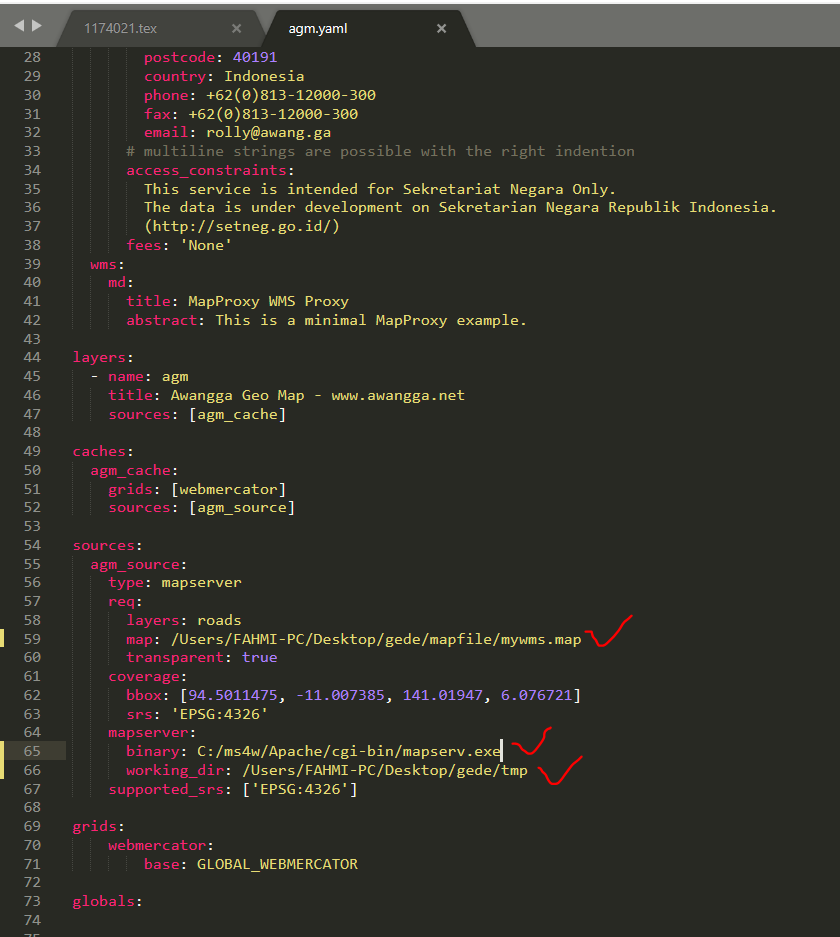
\includegraphics[width=4cm]{figures/1174021/5/4.png}
		\centering
		\caption{Ubah binary dan working dir}
    \end{figure}

    \item Disini boleh menggunakan CMD namun jika gagal boleh menggunakan Anaconda Promt sebagai administrator, pip install pyproj atau conda install pyproj, disini saya menggunakan Anaconda Prompt
    \hfill\break
    \begin{figure}[H]
		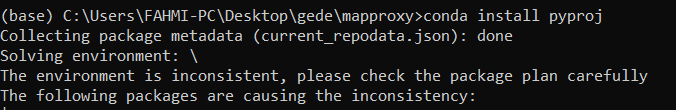
\includegraphics[width=4cm]{figures/1174021/5/5.png}
		\centering
		\caption{Install Pyproj}
    \end{figure} 



    \item Jangan lupa install libproj melalui Anaconda
    \hfill\break
    \begin{figure}[H]
        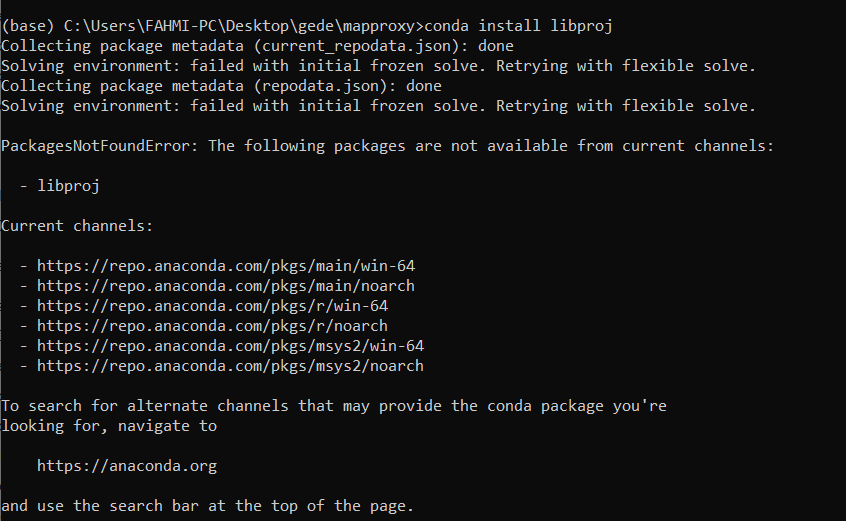
\includegraphics[width=4cm]{figures/1174021/5/6.png}
        \centering
        \caption{Install Libproj}
    \end{figure}

    \end{enumerate}


\subsection{Pengujian}
\begin{enumerate}
    \item Untuk melakukan pengujian bisa dengan menggunakan perintah mapproxy-util serve-develop mapproxy.yaml -b 0.0.0.0:8181 pada Anaconda Prompt
    \hfill\break
    \begin{figure}[H]
		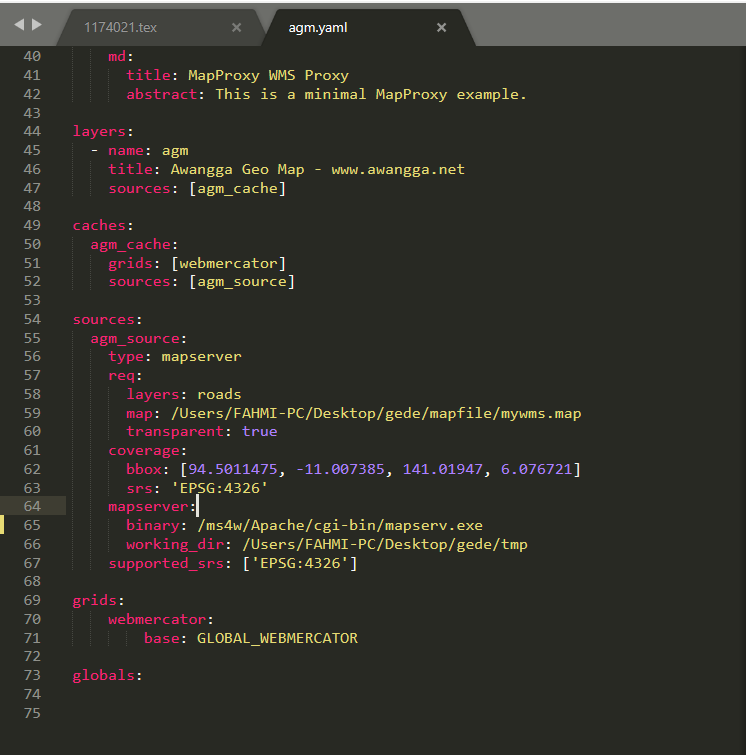
\includegraphics[width=4cm]{figures/1174021/5/7.png}
		\centering
		\caption{Konfigurasi untuk menjalankan mapproxy}
    \end{figure}

    \item Kemudian jalankan di browser http://127.0.0.1:8181/
    \hfill\break
    \begin{figure}[H]
		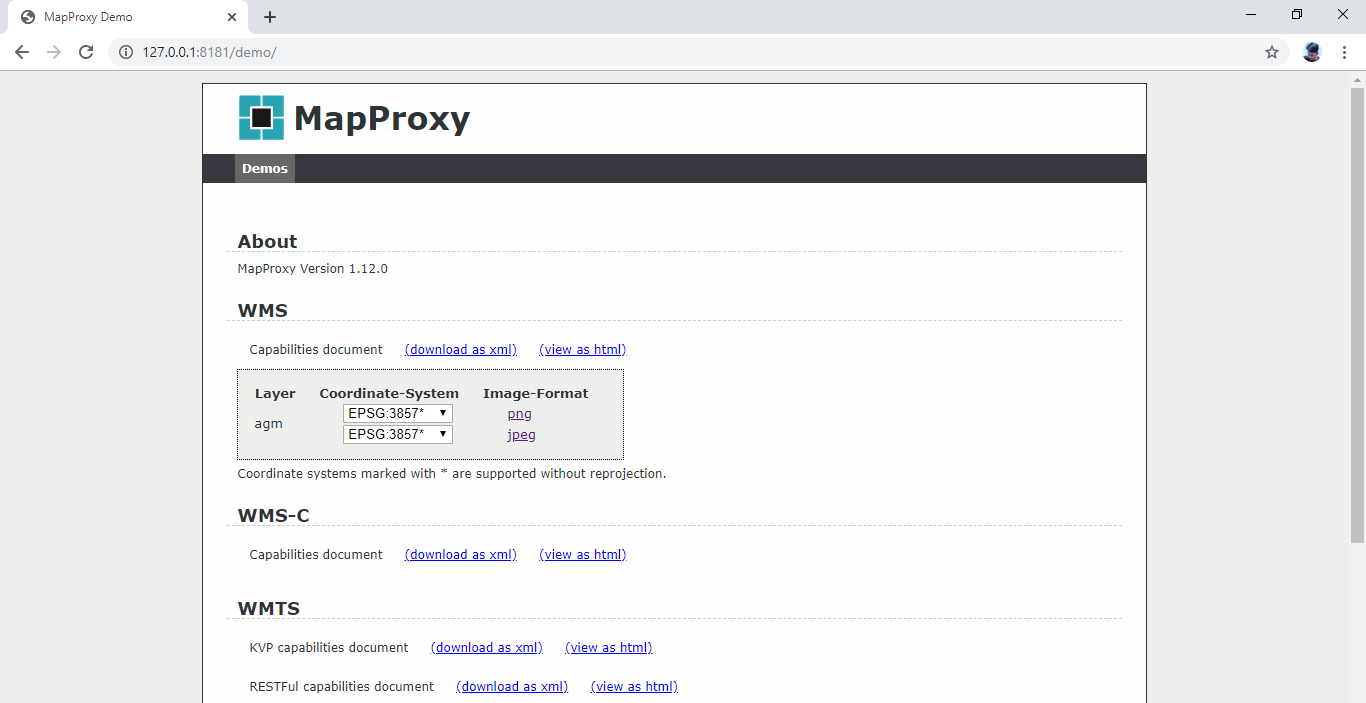
\includegraphics[width=4cm]{figures/1174021/5/8.png}
		\centering
		\caption{Hasil pada Web Browser}
    \end{figure}

\end{enumerate}


\subsection{Plagiarisme}
 \begin{figure}[H]
        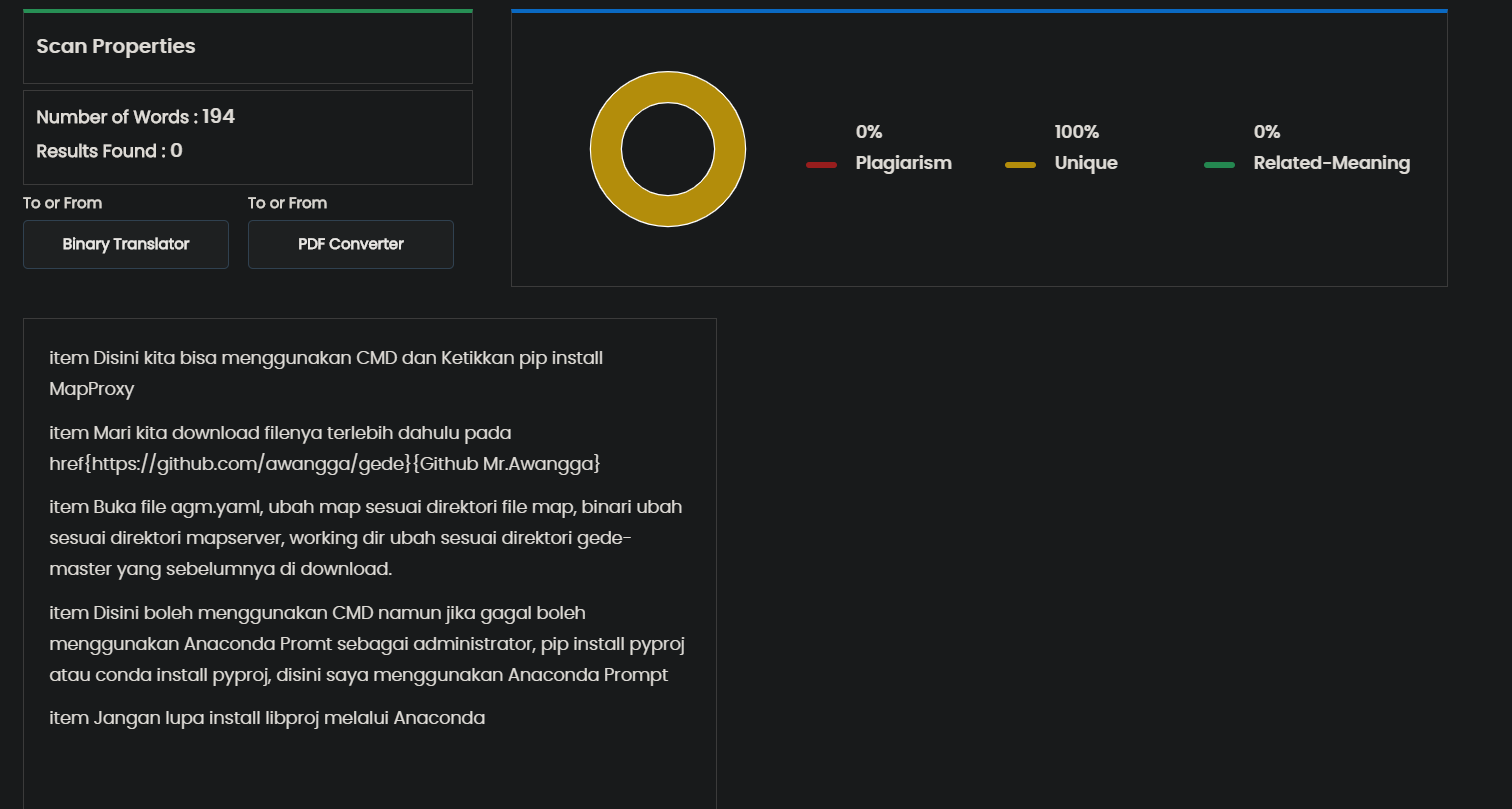
\includegraphics[width=4cm]{figures/1174021/5/plagiat.png}
        \centering
        \caption{No plagiat}
    \end{figure}

\subsection{Link Youtube}
\href{https://www.youtube.com/watch?v=iYgXYX3VbWw}{Klik Disini}